\chapter{Anomaliedetektion}\label{ch:anomaliedetektion}
Anomaliedetektion beschreibt die Aufgabe, Trends, Muster und Punkte in einem Datensatz zu finden, die nicht dem Normalzustand
entsprechen~\cite{Chandola2009}. Anders gesagt lautet das Ziel: die Punkte finden, die sich von den anderen Punkten im Datensatz
stark unterscheiden~\cite[Kap.~10]{Tan2014}. Diese andersartigen Datenpunkte oder -sequenzen werden in der Regel als Anomalie,
Ausreißer oder Ausnahmen bezeichnet, wobei Anomalie der geläufigste Begriff ist. Anomaliedetektion findet große Verwendung in
verschiedenen Anwendungsbereichen, wie z.~B.~in der Netzwerktechnik zur Erkennung von potenziellen Angriffen durch Eindringlinge
in ein Netzwerk anhand von ungewöhnlichem Traffic~\Cite{Bernacki2015}. Auch in der Medizin können nach einem Elektrokardiogramm
(\textit{EKG}) durch Anomaliedetektion Herzrhythmusstörungen erkannt werden~\cite{Chuah2007}, genau wie eine Bank ein Interesse
an Anomalien im Kreditkartenverhalten ihrer Kunden hat, um Betrugsfälle zu erkennen~\cite{Jiang2023, CeronmaniSharmila2019}.

Die simpelste Herangehensweise zur Erkennung von Anomalien ist die, dass zuerst definiert wird, welche Punkte im Datensatz normalem
Verhalten entsprechen und alle davon abweichenden Punkte als Anomalie zu kennzeichnen. Doch so einfach die Herangehensweise wirkt,
so anfällig ist sie auch für Fehler. Dabei heben sich einige Herausforderungen hervor.

Zum Einen die Frage, wo genau die Grenze zwischen normalem und anomalem Verhalten liegen soll. Eine Region zu definieren, die jeden 
möglichen normalen Punkt beinhaltet und jedmöglichen anomalen Punkt ausschließt, ist nicht trivial und oft nicht präzise durchführbar.
So ist es durchaus möglich, dass in manchen Fällen anomale Punkte als normal bezeichnet werden, und normale Punkte als anomal, je
nachdem, wo die Grenze liegt.

Es stellt sich ebenfalls die Frage, ob eine Anomalie einer binären Natur unterliegt: Entweder es handelt sich um eine Anomalie oder
einen Normalzustand. Doch die Wahrheit liegt oft in der Mitte. Weicht ein Punkt oder eine Sequenz bereits nur leicht vom Normal ab,
so kann es bereits erste Hinweise auf mögliches zukünftiges anomales Verhalten in einer Zeitserie geben, bevor sich solche Datenpunkte
als Anomalie zeigen. Deshalb ist es hilfreich, charakterisieren zu können, wie weit der Punkt oder die Sequenz
vom Normal abweicht. Diese Charakterisierung kann dabei als \textit{Anomaly Score} bezeichnet werden und beispielsweise eine Dezimalzahl
zwischen 0 und 1 sein.

Normalzustände sind in Zeitserien oft zeitvariant und daher schwer festzuhalten bei einer kontinuierlichen Datenaufzeichnung.
Zudem sind Normalzustände und Abweichungen davon in unterschiedlichen Bereichen auch unterschiedlich signifikant. Während beim
menschlichen Körper eine geringe Abweichung der Körpertemperatur bereits gravierend sein kann, ist die gleiche relative Abweichung
in einer anderen Domäne wie in einem Aktienkurs weniger drastisch und unterliegt dementsprechend auch einem Anpassungsbedarf, bevor
es an die Erkennung möglicher Anomalien geht.

Daraus lässt sich direkt zum nächsten Problem übergehen. Die Unterscheidung zwischen globalen und lokalen Anomalien~\cite{Breunig2000}.
Hier ist der Kontext wichtig: Eine Person mit einer Körpergröße von mehr als 2 $m$ ist in ihrer Nachbarschaft sicherlich eine Anomalie,
während sie in einem Basketballteam kaum herausragt~-~im wahrsten Sinne des Wortes. Diese Art der Anomalie wird auch als kontextuelle
Anomalie bezeichnet~\Cite[S.~12]{Wenig2024}.

\section{Anomaliearten}
Doch bevor eine Auswahl an geeigneten Verfahren oder Algorithmen zur Anomaliedetektion getroffen wird, muss zuerst verstanden werden,
welche verschiedenen Arten von Anomalien es gibt und wie sich diese voneinander unterscheiden.
Auch wenn Studien zeigen, dass es durchaus Algorithmen gibt, die über mehrere verschiedene Kategorien gut
abschneiden~\cite[S.~30~-~31]{Wenig2024}~\cite{Schmidl2022}, so soll zunächst für jede Kategorie mindestens ein passender Kandidat
gefunden werden. Diese werden dann in einem nächsten Schritt kreuzweise getestet, um auch solche Allrounder entdecken zu können. Dabei
ist auch immer der Kontext der Anwendung wichtig. Wie eingangs erwähnt, sind für verschiedene Tätigkeitsfelder verschiedene
Anforderungen an die Präzision oder Genauigkeit gestellt, weshalb immer die spezifischen Anforderung bedacht werden müssen, und nicht
jeder Algorithmus gleich performant ist über mehrere Datensätze hinweg.

Für die Kategorien wird sich zunächst auf wenige, für diese Arbeit relevante, beschränkt: \textbf{Punkt\-anomalien},
\textbf{Subsequenzanomalien} und \textbf{Korrelationsanomalien}, abgeleitet von Chandola et al.~\cite{Chandola2009}.

\subsection{Punktanomalien}
Ein einzelner Datenpunkt, der stark von den anderen Punkten im Datensatz abweicht, heißt Punkt\-anomalie~\cite{Chandola2009}. Genauer
gesagt, wenn ein Datenpunkt weit außerhalb der Wahrscheinlichkeitsverteilung des Datensatzes liegt, ist er anomal~\Cite[Kap.~10]{Tan2014}.
Punktanomalien können recht leicht erkannt werden, da Punktanomalien stark vom Mittelwert und vom Median des Datensatzes abweichen. Wenn
von Ausreißern gesprochen wird, sind damit typischerweise Punktanomalien gemeint.

Als Beispielszenario dient ein Smart Meter, das den stündlichen Stromverbrauch misst.
In~\hyperref[subfig:smartmeter]{Abb.~\Ref*{subfig:smartmeter}} ist der gemessene Stromverbrauch dargestellt mit einer klar
erkennbaren Punktanomalie am 01.08.~um 18 Uhr. Die Anomalie wird mit bloßem Auge deutlich und kann auch mit statistischen Größen
nachgewiesen werden, wie in~\hyperref[subfig:smartmeter_histogramm]{Abb.~\Ref*{subfig:smartmeter_histogramm}} anhand der
Häufigkeitsverteilung und dem Mittelwert sowie dem Median zu sehen ist. Das Histogramm dient als gute Approximation für die
Wahrscheinlichkeitsverteilung der Messwerte, und zeigt entsprechend die Eindeutigkeit des Ausreißers.

\begin{figure}[!t]
    \centering
    \begin{subfigure}[b]{0.49\linewidth}
        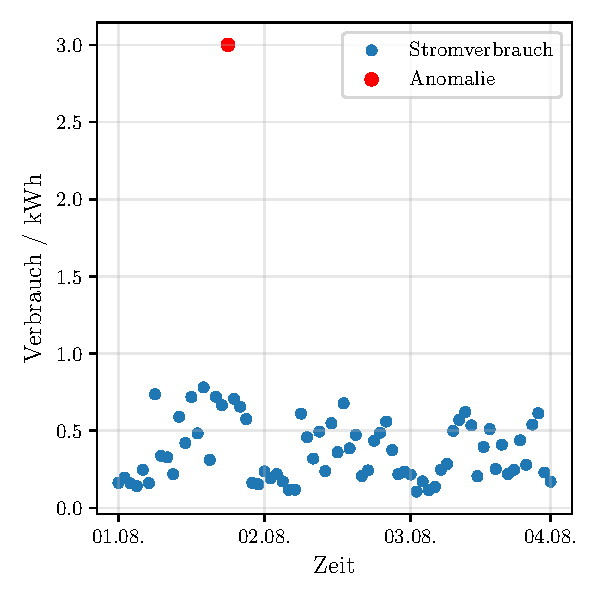
\includegraphics[width=\linewidth]{ch4_anomalien/abbildungen/punktanomalie_bsp.pdf}
        \caption{Stündliche Smart Meter Messdaten}\label{subfig:smartmeter}
    \end{subfigure}
    \begin{subfigure}[b]{0.49\linewidth}
        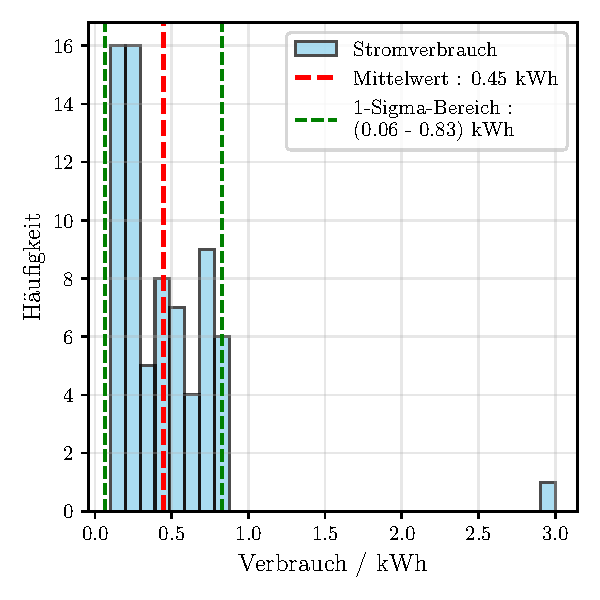
\includegraphics[width=\linewidth]{ch4_anomalien/abbildungen/punktanomalie_hist.pdf}
        \caption{\centering Histogramm des gemessenen Stromverbrauchs}\label{subfig:smartmeter_histogramm}
    \end{subfigure}
    \caption{\centering Beispielszenario einer Punktanomalie: Stromverbrauch eines Haushaltes über den Zeitraum von
    drei Tagen. Anhand des Histogramms wird die Anomalie verdeutlicht.}\label{fig:punktanomalie}
\end{figure}

Um nun eine Aussage treffen zu können, ist es wichtig den Kontext der vorliegenden Daten zu kennen. Wenn Daten für ein weitaus größeres
Zeitfenster vorliegen, z.~B.~für eine Woche oder einen Monat, könnte sich möglicherweise zeigen, dass der hohe Verbrauch öfter und
regelmäßiger vorkommt als im gezeigten Zeitraum von drei Tagen. Ob eine globale oder lediglich eine lokale Anomalie vorliegt, wird
mit einem größeren Datensatz besser erkennbar. Die Anomalie könnte beispielsweise auf das gelegentliche Betreiben einer Sauna im Haus
zurückführbar sein, dann würde es sich lediglich um eine lokale Anomalie handeln und in einem größeren Zeitraum in bestimmten Abständen
öfter vorkommen, und wäre somit keine globale Anomalie~\Cite[Kap.~10]{Tan2014}.

Punktanomalien sind im Kontext dieser Arbeit tendenziell weniger relevant, sollen aber aufgrund ihrer grundsätzlichen Bedeutung bzgl.
Anomaliedetektion als einfachste Kategorie trotzdem beleuchtet werden, um entsprechende Algorithmen, die der Erkennung solcher
Punktanomalien zuzuordnen sind, auch gegenüber anderen Anomalien zu testen.

\subsection{Subsequenzanomalien}

Eine Zeitserie wird gem.~\hyperref[eq:timeseries_set]{Gl.~\Ref*{eq:timeseries_set}} bereits als eine Menge definiert. Demnach wird eine
Subsequenz $S_{i,\,j} = \{\,S_i,\,\dots,\,S_j\,\}\,\subseteq\,S$ von der Zeitserie $S$ umfasst, mit der Länge oder Mächtigkeit
$|\,S_{i,\,j}\,|=j-i+1$ und $|\,S_{i,j}\,|\,\ge\,1$~\cite{Schmidl2022} und stellt somit einen Ausschnitt der urpsrünglichen Zeitserie
dar. Subsequenz\-anomalien sind Muster in Zeitreihen, die von anderen Mustern innerhalb der gleichen Zeitreihe
abweichen~\cite{Chandola2009}\Cite[S.~12]{Wenig2024}. Im Gegensatz zu Punktanomalien beziehen sich Subsequenz\-ano\-malien auf mehrere
konsekutive Datenpunkte, die ein ungewöhnliches Muster bilden. Eine anomale Subsequenz kann also bedeuten, dass die Datenpunkte innerhalb
der Subsequenz Werte in einem normalen, zu erwartenden Bereich annehmen, aber der zu Grunde liegende Trend ungewöhnlich
ist~\cite{Chandola2009}\cite[S.~17]{Boniol2021}. Solche ungewöhnlichen oder einzigartigen Trends und Entwicklungen können auf zukünftig
auftretende Probleme hindeuten, die sonst unentdeckt bleiben würden.

\begin{figure}[H]
    \centering
    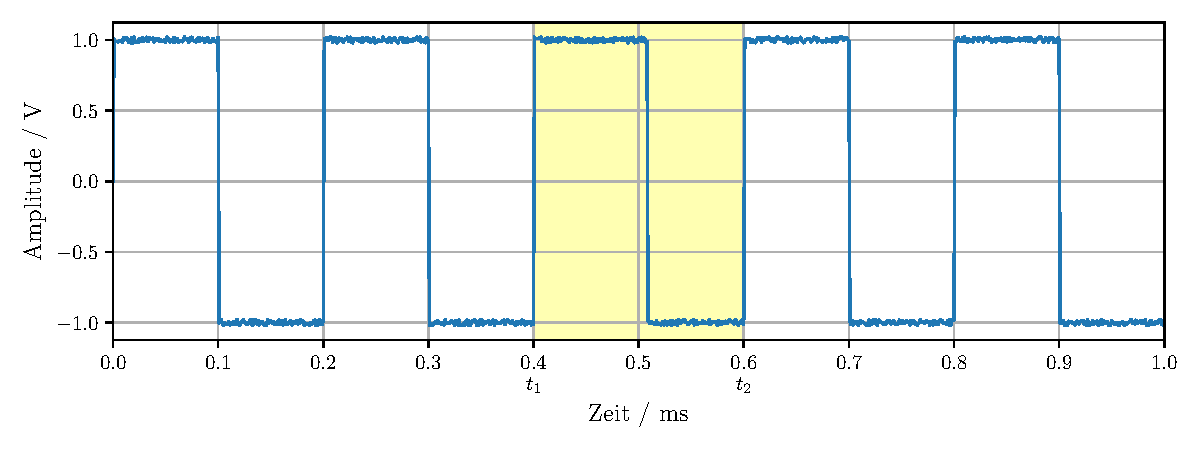
\includegraphics[width=\linewidth]{ch4_anomalien/abbildungen/subsequenz_anomalie.pdf}
    \caption{\centering Einfaches Beispiel einer Subsequenzanomalie: Rechteckspannung, die zwischen -1 und +1 $V$ oszilliert mit einer
    Frequenz von 5 $kHz$. Auffällig ist die Periode zwischen $t_1=0.4\,ms$ und $t_2=0.6\,ms$, bei der eine verspätete abfallende Flanke zu
    beobachten ist.}
~\label{fig:subsequenz_rect}
\end{figure}

Das Beispiel in~\hyperref[fig:subsequenz_rect]{Abb.~\Ref*{fig:subsequenz_rect}} zeigt eine sichtbare Subsequenzanomalie, die verspätete
abfallende Flanke einer gemessenen Rechteckspannung. Das Muster zwischen $t_1$ und $t_2$ ist also merklich anders verglichen zu den
restlichen 0,2 $ms$ langen Perioden und daher eine Anomalie.

Bei der Analyse von EKG Daten spielen Subsequenzanomalien eine wichtige Rolle und können wertvolle Rückschlüsse auf die Herzgesundheit
liefern~\cite{Chuah2007}.~\hyperref[fig:ekg_herzerkrankung]{Abb.~\Ref*{fig:ekg_herzerkrankung}} zeigt EKG-Daten eines Patienten mit
monomorpher ventrikulärer Tachykardie. Diese kann zu Kammerflimmern übergehen, welches unbehandelt sogar zu einem Herzstillstand
führen kann~\cite{ekgecho}\Cite[S.~131~ff.]{Davies2015}.

\begin{figure}[h]
    \centering
    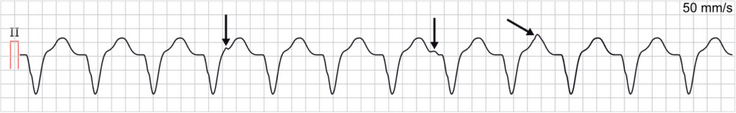
\includegraphics[width=\linewidth]{ch4_anomalien/abbildungen/ventrikulaere_tachykardie.png}
    \caption{EKG Kanal mit Diagnose: Ventrikuläre Tachykardie~\cite{ekgecho}}
~\label{fig:ekg_herzerkrankung}
\end{figure}

Sichtbar sind die einzelnen Unregelmäßigkeiten im EKG Verlauf. Die Pfeile kennzeichnen die sog. P-Wellen, die Informationen darüber
liefern, dass Vorhöfe und Herzkammern nicht synchron schlagen~\cite{ekgecho}\Cite[S.~31~f.]{Davies2015}. Durch die Irregularitäten lässt
sich also erkennen, dass für den untersuchten Patienten eine Behandlung notwendig ist und betont die Wichtigkeit, diese Anomalien zu
erkennen, um wesentlich Schlimmeres zu verhindern.

Darin liegt auch eine der Herausforderungen der Subsequenzanomaliedetektion: Ab wann ist ein Trend, der so noch nicht aufgetreten ist,
Grund genug, um Maßnahmen zu ergreifen? Es bedarf also menschlicher Expertise zur Einordnung und Interpretation von Anomalien, eben wie
bei EKG Daten.

\subsection{Korrelationsanomalien}

Während Punkt- und Subsequenzanomalien sowohl für univariate als auch multivariate Datensätze und Zeitserien auftreten können, sind
Korrelationsanomalien nur möglich bei zwei oder mehr Dimensionen einer Zeitreihe und betrachten die Interaktionen zwischen
verschiedenen Kanälen. Von einer Korrelationsanomalie spricht man bei Abweichungen dieser Beziehung zwischen zwei oder mehreren
Kanälen~\cite[S.12-13]{Wenig2024}~\cite{Wenig2024a}.

\begin{figure}[H]
    \centering
    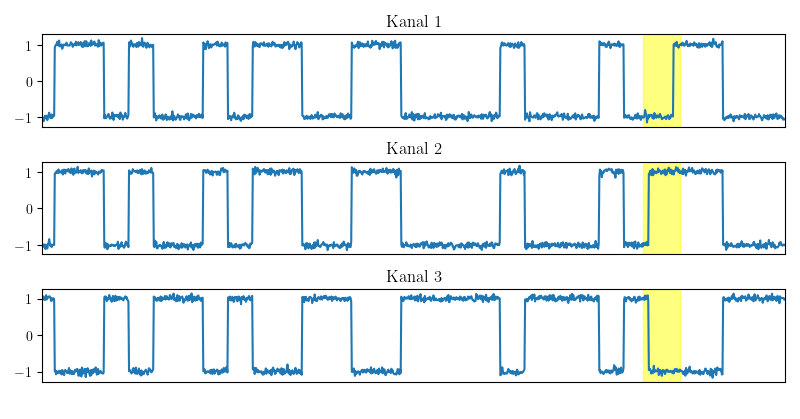
\includegraphics[width=\linewidth]{ch4_anomalien/abbildungen/korrelationsanomalie.png}
    \caption{\centering Korrelationsanomalie zwischen Kanal 1 und den Kanälen 2 und 3 im gelb markierten Bereich. Quelle: Datensatz
        \textit{CoMuT}~\cite{NaumannCoMuT}}
~\label{fig:correlation_Anomaly}
\end{figure}

Im vorliegenden Beispiel in~\hyperref[fig:correlation_Anomaly]{Abb.~\Ref*{fig:correlation_Anomaly}} ist ein Auszug aus dem Datensatz
\textit{CoMuT}~- \textbf{Co}rrelated \textbf{Mu}lti\-variate \textbf{T}ime Series~\cite{NaumannCoMuT} dargestellt. Die Zeitreihe besteht
aus drei Kanälen, die zu zufälligen Zeitpunkten sprungartig ihren Wert zwischen $-$1 und 1 wechseln und jeweils leicht verrauscht sind.
Kanal 1 und 2 sind stark korreliert, während Kanal 3 stark antikorreliert zu den beiden ersten Kanälen ist. Diese Korrelation wird im
markierten Bereich verletzt, da Kanal 1 später springt als die anderen beiden Kanäle~$-$~somit liegt eine Korrelations\-anomalie vor.

\section{Algorithmen zur Anomaliedetektion}
Um nun eine geeignete Auswahl an Algorithmen zu treffen